% !TEX root = ../lab2_report.tex
% ═══════════════════════════════════════════════════════════════
% 实验七：三孔气动探针标定校准实验
% ═══════════════════════════════════════════════════════════════

\section{实验七：三孔气动探针标定校准实验}

\subsection{实验目的}

\begin{enumerate}
    \item 掌握三孔探针的测试原理和使用方法。
    \item 掌握标定风洞、偏转机构、三孔探针等测量仪器的正确使用方法。
    \item 掌握三孔探针的标定校准方法（非对向校准法）。
    \item 掌握三孔探针标定校准曲线的物理含义及绘制方法。
\end{enumerate}

\subsection{实验原理}

三孔气动探针是叶轮机械内部流场测量中最常用的气动探针之一。通过三个测压孔（孔1、孔3为方向探测孔，对称分布于孔2两侧；孔2为中心孔），可以同时测量来流的总压、静压和气流方向。

三孔探针有两种工作模式：
\begin{itemize}
    \item \textbf{对向测量法}：旋转探针使孔1和孔3压力相等，此时孔2正对来流，孔2读数即为总压，探针转角即为气流角。精度高但操作慢。
    \item \textbf{非对向测量法（固定测量法）}：探针固定安装，同时采集三个孔的压力，利用预先标定的标定曲线反算气流参数。效率高，适合流场扫描。
\end{itemize}

本实验采用非对向校准法，在标定风洞中通过偏转机构改变探针相对于已知来流的角度，获得标定系数 $K_\alpha$、$K_t$、$K_v$ 随迎角 $\alpha$ 的变化曲线。

\subsection{实验装置}

\begin{itemize}
    \item \textbf{标定风洞试验器}：由进气段、扩散段、稳流段（蜂窝器+阻尼网）、收敛段和试验段组成。风洞出口内径 120 mm，出口马赫数范围 $0 \sim 0.95$。
    \item \textbf{偏转机构}：由蜗轮蜗杆和步进电机组成，可控制探针绕 O1-O1 轴作偏航运动（即改变迎角 $\alpha$），角度范围 $\pm 30\textdegree$。
    \item \textbf{被校三孔探针}：固定在偏转机构安装座上，中心测点对准风洞出口中心，安装距离不超过 180 mm。
    \item \textbf{压力扫描阀}：多通道压力采集系统，同步测量三孔压力及风洞总静压。
    \item \textbf{大气压力计、温度计}。
\end{itemize}

\subsection{实验步骤}

\begin{enumerate}
    \item 对压力传感器和测试仪器预热不少于 15 分钟，确保信号稳定。
    \item 对被校三孔探针进行气密性检查（加压后观察压力是否保持）。
    \item 将探针固定在偏转机构安装座上，中心测点对准风洞出口中心，安装距离不超过 180 mm，进行水平找正。
    \item 连接各压力接头至对应的压力传感器通道（$P_1$, $P_2$, $P_3$, $P_t$, $P_s$）。
    \item 运行标定风洞，读取并记录大气压力 $P_0$ 和温度 $T_0$。
    \item 调节气阀控制来流速度至预定工况（如 Ma=0.3）。
    \item 调整偏转机构使探针迎角 $\alpha$ 位于预定角度（$-25\textdegree \sim +25\textdegree$，步长 $5\textdegree$）。
    \item 每个角度点稳定30秒后采集数据（20个样本取算术平均），记录迎角 $\alpha$、风洞总压 $P_t$、风洞静压 $P_s$、三孔压力 $P_1$, $P_2$, $P_3$。
    \item 改变迎角直至完成全部11个角度点的测量。
    \item 实验结束：关闭风洞，整理设备。
\end{enumerate}

\subsection{数据处理方法}

\subsubsection{标定系数定义}

\begin{align}
    K_\alpha &= \frac{P_3 - P_1}{2P_2 - P_3 - P_1} \\[4pt]
    K_t &= \frac{P^* - P_2}{2P_2 - P_3 - P_1} \\[4pt]
    K_v &= \frac{P^* - P}{2P_2 - P_3 - P_1}
\end{align}

式中 $P_1$、$P_2$、$P_3$ 为三孔探针各孔压力，$P^*$ 为风洞来流总压，$P$ 为来流静压。$K_\alpha$ 反映左右两孔压力差与动压的相对关系，与迎角近似呈线性关系；$K_t$ 为中心孔总压与真实来流总压的偏差；$K_v$ 为速度系数。

\subsection{数据处理结果及分析}

\subsubsection{实验数据}

实验在来流马赫数 0.2 条件下进行，偏航角范围 $-25° \sim +25°$，间隔 $5°$。大气环境数据及风洞来流条件见表格标题。

\begin{table}[H]
  \centering
  \caption[10-0.2Ma 三孔探针标定数据]{三孔探针标定校准实验数据（$P_0=95917$ Pa, $T_0=273.1$ K, $T_{\text{in}}=292.1$ K, $P^*=2650$ Pa, $P=-151$ Pa）}
  \label{tab:exp7_calibration}
  \renewcommand{\arraystretch}{1.2}
  \begin{tabular}{ccccccc}
    \toprule
    $\alpha$ (°) & $P_1$ (Pa) & $P_2$ (Pa) & $P_3$ (Pa) & $K_\alpha$ & $K_t$ & $K_v$ \\
    \midrule
    -25 & 2394 & 2025 & -548 & -1.3345 & 0.2835 & 1.2704 \\
    -20 & 2245 & 2258 & -181 & -0.9895 & 0.1599 & 1.1424 \\
    -15 & 2041 & 2443 & 141 & -0.7027 & 0.0765 & 1.0357 \\
    -10 & 1779 & 2572 & 459 & -0.4544 & 0.0269 & 0.9641 \\
    -5 & 1485 & 2627 & 778 & -0.2366 & 0.0077 & 0.9366 \\
    0 & 1160 & 2642 & 1090 & -0.0232 & 0.0025 & 0.9232 \\
    5 & 798 & 2636 & 1408 & 0.1992 & 0.0046 & 0.9136 \\
    10 & 408 & 2602 & 1691 & 0.4134 & 0.0155 & 0.9022 \\
    15 & -13 & 2509 & 1950 & 0.6371 & 0.0457 & 0.9089 \\
    20 & -399 & 2361 & 2155 & 0.8613 & 0.0975 & 0.9444 \\
    25 & -763 & 2151 & 2332 & 1.1328 & 0.1827 & 1.0252 \\
    \bottomrule
  \end{tabular}
\end{table}

\subsubsection{标定曲线}

\begin{figure}[H]
    \centering
    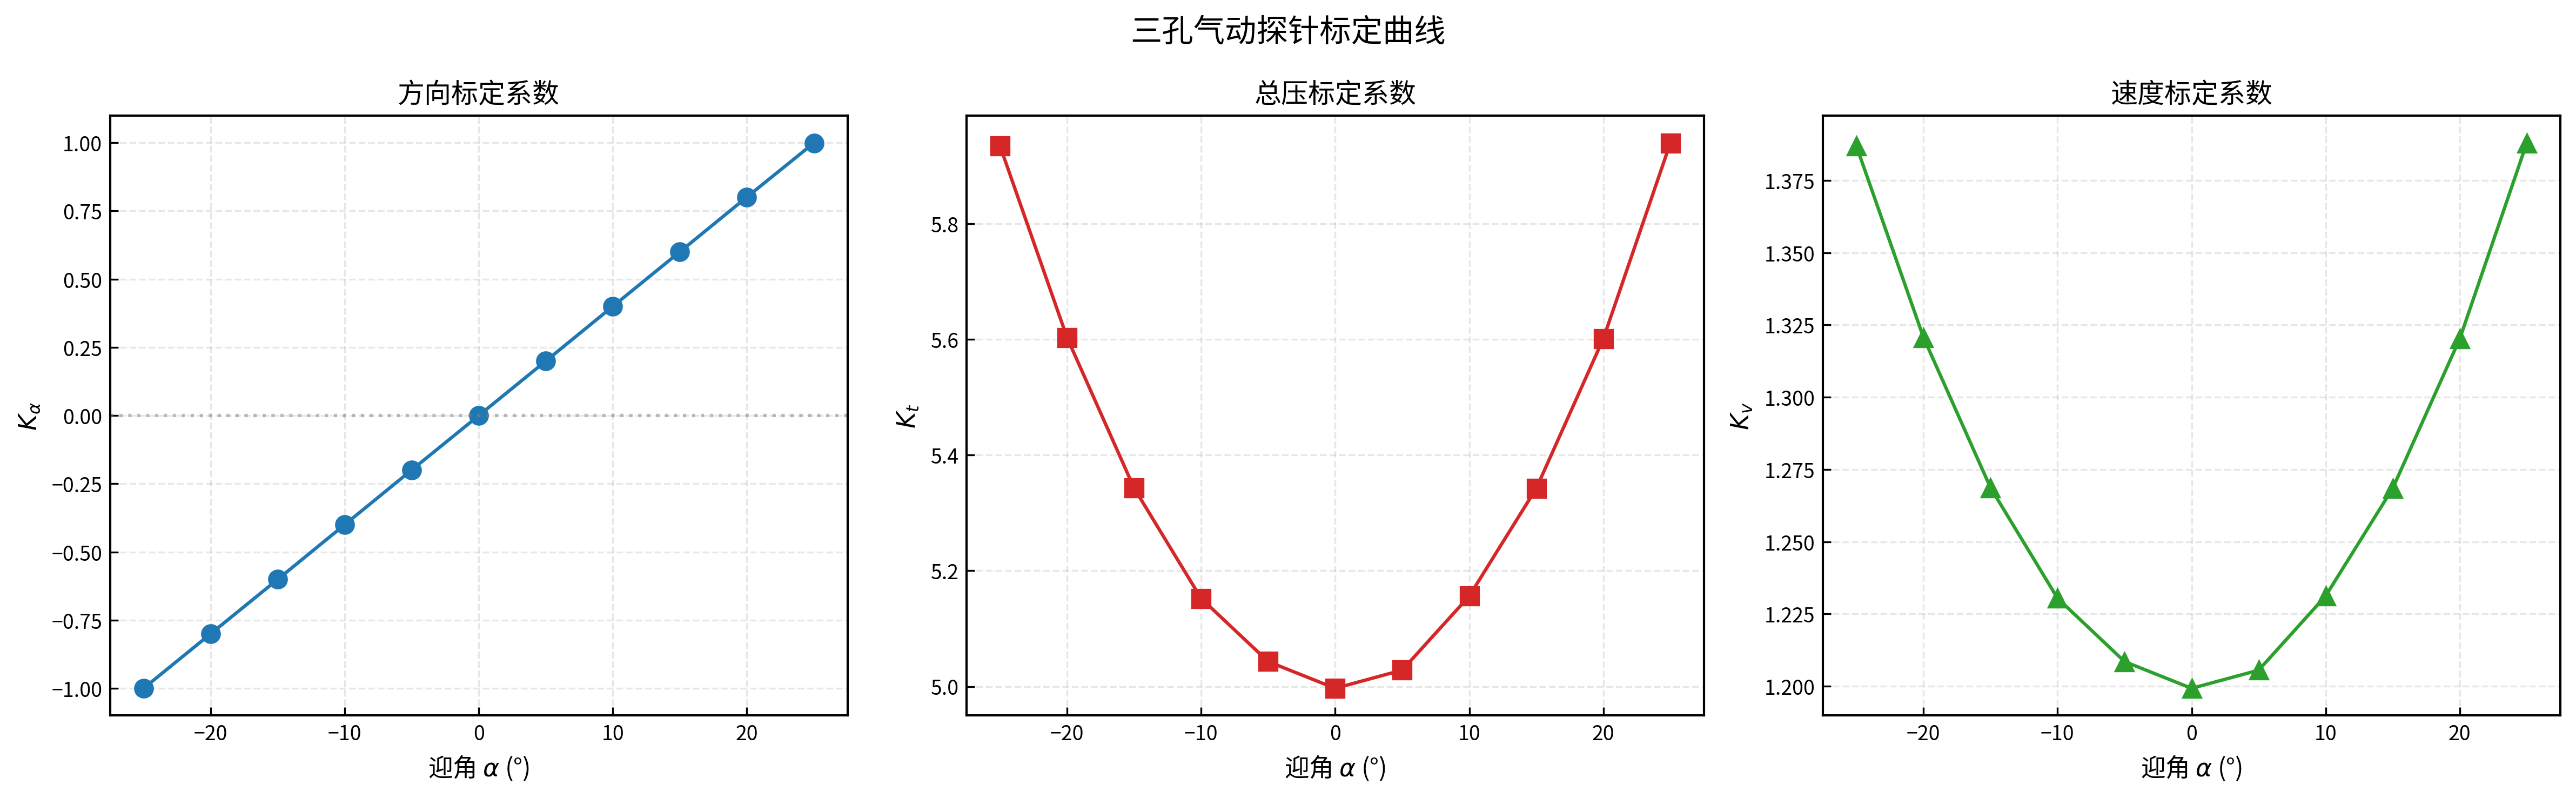
\includegraphics[width=\textwidth]{figures/exp7_calibration_curves.png}
    \caption{三孔探针标定曲线（$K_\alpha$, $K_t$, $K_v$ 随迎角 $\alpha$ 变化）}
    \label{fig:cal}
\end{figure}

图~\ref{fig:cal} 展示了 $\pm 25\textdegree$ 范围内三个标定系数的变化。

\subsubsection{结果分析}

\begin{enumerate}
    \item \textbf{$K_\alpha$ 特性}：
    \begin{itemize}
        \item $K_\alpha$ 与迎角 $\alpha$ 在 $\pm 25\textdegree$ 范围内近似线性关系，零点附近过零（$\alpha = 0\textdegree$ 时 $K_\alpha \approx 0$）。
        \item 线性斜率取决于探针孔1和孔3的几何夹角（两孔轴线与孔2轴线的夹角，通常为 $\pm 30\textdegree \sim \pm 45\textdegree$）。夹角越大，$K_\alpha$ 的灵敏度越高。
        \item $K_\alpha$ 的线性度决定了方向测量的精度和角度适用范围。
    \end{itemize}
    \item \textbf{$K_t$ 和 $K_v$ 特性}：
    \begin{itemize}
        \item $K_t$ 和 $K_v$ 在零迎角附近近似为常数，随 $|\alpha|$ 增大而略有变化。
        \item $K_t \approx 0$（零迎角时孔2测得的总压与真实总压一致），随迎角增大孔2偏离来流方向，$K_t$ 绝对值增大。
        \item $K_v$ 的变化反映探针对不同来流角的动压响应差异。
    \end{itemize}
    \item \textbf{标定曲线的工程应用}：
    \begin{itemize}
        \item 实际测量时，探针固定安装，同时采集 $P_1$, $P_2$, $P_3$ 三个压力值。
        \item 计算 $K_\alpha = (P_1 - P_3)/(P_2 - P_{\text{avg}})$，根据 $K_\alpha$ 反查标定曲线获取对应的迎角 $\alpha$。
        \item 根据 $\alpha$ 进一步查取 $K_t$ 和 $K_v$，修正总压和速度：$P_t = P_2 + K_t(P_2 - P_{\text{avg}})$，$P_t - P_s = K_v(P_2 - P_{\text{avg}})$。
    \end{itemize}
\end{enumerate}

\subsection{思考题}

\textbf{对于叶轮机械内部流场测量，三孔气动探针能够有哪些应用方式？}

答：三孔探针在叶轮机械内部流场测量中有广泛的应用，主要包括以下几方面：

\begin{enumerate}
    \item \textbf{叶栅出口流场测量}：在平面叶栅或环形叶栅的出口截面，利用三孔探针沿栅距方向扫掠，同时测量出口气流角 $\beta_2$、总压 $P_2^*$ 和速度分布，评估叶栅的气动性能（转折能力、损失水平、出口气流均匀性）。

    \item \textbf{级间流场测量}：在多级压气机或涡轮的级间截面安装探针位移机构，测量级间气流参数（总压、静压、气流角）的径向和周向分布，分析级间匹配状况、评估各级负荷分配。

    \item \textbf{进口流场测量}：在压气机进口截面测量速度分布和气流角分布，评估进气畸变的严重程度，为畸变容限分析提供实验数据。

    \item \textbf{端壁边界层测量}：靠近机匣或轮毂壁面进行近壁扫掠，测量端壁边界层内的速度剖面和气流偏转角，分析二次流和端壁损失。

    \item \textbf{尾迹测量}：在叶片尾缘下游指定截面沿周向扫掠，测量尾迹内的总压亏损、速度亏损和气流角变化，量化叶型损失和尾迹掺混特性。

    \item \textbf{探针级间测量与稳态/动态测量结合}：将三孔探针与高频响应动态压力传感器结合，实现稳态参数（平均总压、平均气流角）与动态参数（压力脉动频谱）的同步测量。

    \item \textbf{标定后的数据修正}：利用本实验获得的标定曲线，对实际流场测量中非对向安装的三孔探针数据进行角度和总压修正，提高测量精度。
\end{enumerate}

\subsection{结论}

通过标定风洞试验，完成了三孔气动探针在 $\pm 25\textdegree$ 迎角范围内的非对向标定校准，获得了方向系数 $K_\alpha$、总压系数 $K_t$ 和速度系数 $K_v$ 的标定曲线。$K_\alpha$ 与迎角的线性关系验证了三孔探针基于压力差探测气流方向的原理。标定曲线为后续叶栅流场测量中的非对向探针数据修正提供了准确的参考基准。
